\documentclass[a4paper, 11pt]{article}
\usepackage{amsmath}
\usepackage{graphicx}
\usepackage{geometry}
\usepackage{listings}
\geometry{scale=0.8}
\linespread{1.5}
\usepackage{hyperref}

\title{	
\normalfont \normalsize
\textsc{School of Data and Computer Science, Sun Yat-sen University} \\ [25pt] %textsc small capital letters
\rule{\textwidth}{0.5pt} \\[0.4cm] % Thin top horizontal rule
\huge  E04 Futoshiki Puzzle ( Forward Checking)\\ % The assignment title
\rule{\textwidth}{2pt} \\[0.5cm] % Thick bottom horizontal rule
\author{19214808 Yikun Liang}
\date{\normalsize\today}
}

\begin{document}
\maketitle
\tableofcontents
\newpage

\section{Futoshiki}
Futoshiki is a board-based puzzle game, also known under the name Unequal. It is playable on a square board having a given fixed size ($4\times4$ for example).

The purpose of the game is to discover the digits hidden inside the board's cells; each cell is filled with a digit between 1 and the board's size. On each row and column each digit appears exactly once; therefore, when revealed, the digits of the board form a so-called Latin square.

At the beginning of the game some digits might be revealed. The board might also contain some inequalities between the board cells; these inequalities must be respected and can be used as clues in order to discover the remaining hidden digits.

Each puzzle is guaranteed to have a solution and only one.

You can play this game online: \url{http://www.futoshiki.org/}.
\begin{figure}[h]
  \centering
  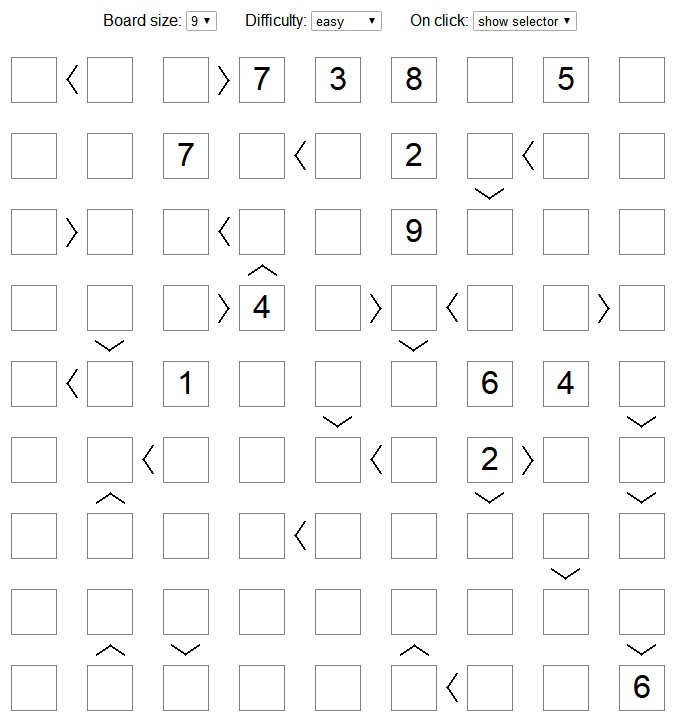
\includegraphics[width=7.5cm]{Pic/futoshiki1}
  \qquad
  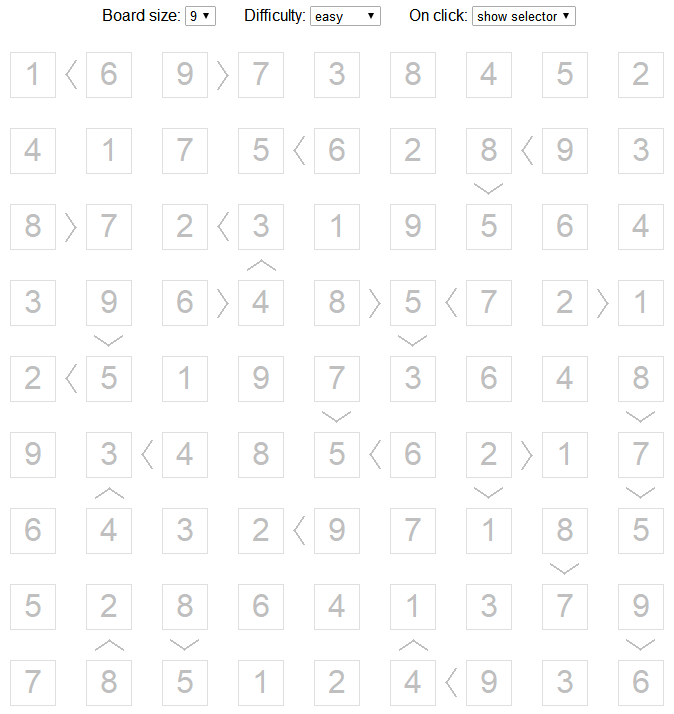
\includegraphics[width=7.5cm]{Pic/futoshiki2}
  \label{fig:puzzle}
  \caption{An Futoshiki Puzzle}
\end{figure}

\section{Tasks}


\begin{enumerate}
\item Please solve the above Futoshiki puzzle ( Figure \ref{fig:puzzle} ) with forward checking algorithm.
\item Write the related codes and take a screenshot of the running results in the file named \textsf{E04\_YourNumber.pdf}, and send it to \textsf{ai\_201901@foxmail.com}.

\end{enumerate}
\section{Codes}
\section{Results}


%\clearpage
%\bibliography{E:/Papers/LiuLab}
%\bibliographystyle{apalike}
\end{document} 
%%% Local Variables:
%%% mode: latex
%%% TeX-master: t
%%% End:
